\documentclass[tikz,border=3pt]{standalone}
\usepackage{amsmath,amssymb}
\usetikzlibrary{arrows.meta,positioning,calc,fit,backgrounds,decorations.pathreplacing,shapes.geometric}
\begin{document}
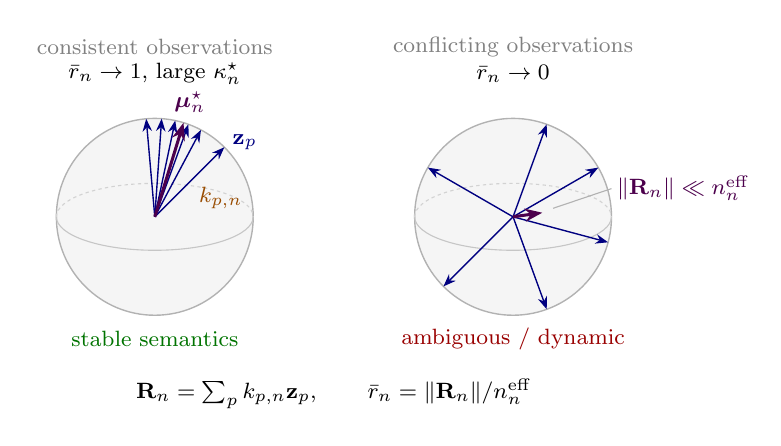
\begin{tikzpicture}[font=\footnotesize,
  obs/.style={-{Stealth[length=1.6mm]}, line width=0.5pt, blue!50!black},
  res/.style={-{Stealth[length=2.2mm]}, line width=1.1pt, violet!60!black}]

\def\R{1.25}

% ---------------- LEFT sphere: consistent observations ----------------
\begin{scope}
  \draw[gray!60, fill=gray!8, line width=0.5pt] (0,0) circle (\R);
  \draw[gray!45, line width=0.4pt]
    (-\R,0) arc[start angle=180, end angle=360, x radius=\R, y radius=0.34*\R];
  \draw[gray!35, line width=0.4pt, dash pattern=on 1.2pt off 1.2pt]
    (-\R,0) arc[start angle=180, end angle=0, x radius=\R, y radius=0.34*\R];
  % clustered unit observations
  \foreach \a in {45,62,70,78,86,95} \draw[obs] (0,0) -- (\a:\R);
  % posterior mean direction (resultant nearly unit length)
  \draw[res] (0,0) -- (73:\R);
  \node[violet!60!black, inner sep=1pt] at (73:1.52) {$\boldsymbol{\mu}^\star_n$};
  % example observation + kernel weight
  \node[blue!50!black, anchor=west, inner sep=1pt] at (45:1.34) {$\mathbf{z}_p$};
  \node[orange!60!black, anchor=north west, inner sep=1pt]
    at (0.52,0.42) {$k_{p,n}$};
  % headers / annotations
  \node[gray] at (0,2.16) {consistent observations};
  \node at (0,1.82) {$\bar r_n\to 1$, large $\kappa^\star_n$};
  \node[green!45!black] at (0,-1.55) {stable semantics};
\end{scope}

% ---------------- RIGHT sphere: conflicting observations ----------------
\begin{scope}[shift={(4.55,0)}]
  \draw[gray!60, fill=gray!8, line width=0.5pt] (0,0) circle (\R);
  \draw[gray!45, line width=0.4pt]
    (-\R,0) arc[start angle=180, end angle=360, x radius=\R, y radius=0.34*\R];
  \draw[gray!35, line width=0.4pt, dash pattern=on 1.2pt off 1.2pt]
    (-\R,0) arc[start angle=180, end angle=0, x radius=\R, y radius=0.34*\R];
  % widely spread unit observations (some near-opposite);
  % their true vector sum points at ~2deg with |R|/6 ~ 0.16
  \foreach \a in {30,70,150,225,290,345} \draw[obs] (0,0) -- (\a:\R);
  % short resultant (drawn along the true sum direction)
  \draw[res] (0,0) -- (8:0.30*\R);
  \draw[gray!60, line width=0.4pt] (12:0.52) -- (16:1.30);
  \node[violet!60!black, anchor=west, inner sep=1pt] at (16:1.33)
    {$\lVert\mathbf{R}_n\rVert\ll n^{\mathrm{eff}}_n$};
  % headers / annotations
  \node[gray] at (0,2.16) {conflicting observations};
  \node at (0,1.82) {$\bar r_n\to 0$};
  \node[red!60!black] at (0,-1.55) {ambiguous / dynamic};
\end{scope}

% ---------------- sufficient statistics ----------------
\node at (2.275,-2.25)
  {$\mathbf{R}_n=\sum_p k_{p,n}\mathbf{z}_p, \qquad \bar r_n=\lVert\mathbf{R}_n\rVert / n^{\mathrm{eff}}_n$};

\end{tikzpicture}
\end{document}
